% THIS IS SIGPROC-SP.TEX - VERSION 3.1
% WORKS WITH V3.2SP OF ACM_PROC_ARTICLE-SP.CLS
% APRIL 2009
%
% It is an example file showing how to use the 'acm_proc_article-sp.cls' V3.2SP
% LaTeX2e document class file for Conference Proceedings submissions.
% ----------------------------------------------------------------------------------------------------------------
% This .tex file (and associated .cls V3.2SP) *DOES NOT* produce:
%       1) The Permission Statement
%       2) The Conference (location) Info information
%       3) The Copyright Line with ACM data
%       4) Page numbering
% ---------------------------------------------------------------------------------------------------------------
% It is an example which *does* use the .bib file (from which the .bbl file
% is produced).
% REMEMBER HOWEVER: After having produced the .bbl file,
% and prior to final submission,
% you need to 'insert'  your .bbl file into your source .tex file so as to provide
% ONE 'self-contained' source file.
%
% Questions regarding SIGS should be sent to
% Adrienne Griscti ---> griscti@acm.org
%
% Questions/suggestions regarding the guidelines, .tex and .cls files, etc. to
% Gerald Murray ---> murray@hq.acm.org
%
% For tracking purposes - this is V3.1SP - APRIL 2009

\documentclass{sig-alternate-10pt}

%
\def\sharedaffiliation{%
\end{tabular}
\begin{tabular}{c}}
%

% use png
\usepackage{graphicx}

%math
\usepackage{amssymb, amsmath}

%algo
\usepackage{algorithm}
\usepackage{algorithmicx}
\usepackage{algpseudocode}

% remove copyright box
\usepackage{etoolbox}
\usepackage{color}
\makeatletter
\patchcmd{\maketitle}{\@copyrightspace}{}{}{}
\makeatother
%

\begin{document}

\title{Chornamo!}

% You need the command \numberofauthors to handle the 'placement
% and alignment' of the authors beneath the title.
%
% For aesthetic reasons, we recommend 'three authors at a time'
% i.e. three 'name/affiliation blocks' be placed beneath the title.
%
% NOTE: You are NOT restricted in how many 'rows' of
% "name/affiliations" may appear. We just ask that you restrict
% the number of 'columns' to three.
%
% Because of the available 'opening page real-estate'
% we ask you to refrain from putting more than six authors
% (two rows with three columns) beneath the article title.
% More than six makes the first-page appear very cluttered indeed.
%
% Use the \alignauthor commands to handle the names
% and affiliations for an 'aesthetic maximum' of six authors.
% Add names, affiliations, addresses for
% the seventh etc. author(s) as the argument for the
% \additionalauthors command.
% These 'additional authors' will be output/set for you
% without further effort on your part as the last section in
% the body of your article BEFORE References or any Appendices.

\numberofauthors{3} %  in this sample file, there are a *total*
% of EIGHT authors. SIX appear on the 'first-page' (for formatting
% reasons) and the remaining two appear in the \additionalauthors section.
%
\author{
% You can go ahead and credit any number of authors here,
% e.g. one 'row of three' or two rows (consisting of one row of three
% and a second row of one, two or three).
%
% The command \alignauthor (no curly braces needed) should
% precede each author name, affiliation/snail-mail address and
% e-mail address. Additionally, tag each line of
% affiliation/address with \affaddr, and tag the
% e-mail address with \email.
%
% 1st. author
\alignauthor
Connie Chen
       \email{cwc009@cs.ucsd.edu}
% 2nd. author
\alignauthor 
Russell Reas
    \email{rreas@cs.ucsd.edu}
% 3rd. author
\alignauthor
Rakesh Varna
       \email{rvarna@cs.ucsd.edu}
\sharedaffiliation
\affaddr{Department of Computer Science and Engineering}\\
\affaddr{University of California, San Diego}
}

% There's nothing stopping you putting the seventh, eighth, etc.
% author on the opening page (as the 'third row') but we ask,
% for aesthetic reasons that you place these 'additional authors'
% in the \additional authors block, viz.
%\additionalauthors{Additional authors: John Smith (The Th{\o}rv{\"a}ld Group,
%email: {\texttt{jsmith@affiliation.org}}) and Julius P.~Kumquat
%(The Kumquat Consortium, email: {\texttt{jpkumquat@consortium.net}}).}
%\date{30 July 1999}
% Just remember to make sure that the TOTAL number of authors
% is the number that will appear on the first page PLUS the
% number that will appear in the \additionalauthors section.

\maketitle
\begin{abstract}
In this report, we implement and evaluate the performance of a Distributed Hash Table (DHT) based on Chord \cite{chord}. In addition to supporting node joining and failure as outlined in the Chord paper, we experiment with synchronous and asynchronous replication strategies based on sharing data with one or more successors.  All code is available on GitHub \cite{github} and written in Python using the Thrift RPC \cite{thrift} framework.
\end{abstract}

% A category with the (minimum) three required fields
%\category{H.4}{Information Systems Applications}{Miscellaneous}
%A category including the fourth, optional field follows...
%\category{D.2.8}{Software Engineering}{Metrics}[complexity measures, performance measures]

\terms{Reliability, Experimentation, Distribution}

\keywords{Distributed Hash Tables, Distributed Key-Value Stores, Consistent Hashing, Chord, Replication, Thrift RPC, Asynchronous Replication} % NOT required for Proceedings

\section{Introduction}
Distributed Hash Tables (DHTs) serve as decentralized key-value stores that can scale well and are fault-tolerant. Each participating node is responsible for storing a set of keys and their corresponding values. DHTs are known for their fast, $O(\log N)$ key lookups \cite{chord}.

The remainder of the report is structured as follows: Section 2 briefly describes Chord, a peer to peer lookup protocol that our implementation is based on. Section 3 describes the different lookup and replication strategies that we have implemented. We discuss the design of our experiments in Section 4. In Section 5, we analyze and discuss the results of our experiments. We conclude in section 6.

\section{Chord} 
Chord is a peer-to-peer lookup protocol that maps a given key onto a node. It uses consistent hashing \cite{consistent-hashing} to assign keys to the nodes \cite{chord}. Consistent hashing tends to balance load with each node receiving approximately the same fraction of keys. In order to scale to large number of nodes, a given node should store minimal amount of information about the other nodes in the system. In an N-node system using Chord, any given node maintains information about only $O(\log n)$ other nodes and the lookup involves only $O(\log N)$ messages. Note that this is only for faster lookups. For correctness, it is sufficient to maintain a pointer to the next node along the circle.
As nodes join and leave the system, the `routing' information stored at any given might become stale. This results in degraded performance, yet does not affect correctness. Chord only requires that a given node maintain the correct information about its successor, the next node on the circle (clock-wise), considering the nodes being arranged in a circle, as per consistent hashing. Replication and storing values associated with the keys is handled in the higher level application.
\subsection{Efficient lookups}
The nodes in Chord maintain a `finger-table', with the $i^{th}$ entry in the table pointing to the successor of the key $(n + 2^{i - 1}) \mod 2^m, \; 1 \leq i \leq m$, where $m$ is the number of bits in the output of the hash function used. Given that node is likely to be within a distance of $2^m/N^2$ of any other node\footnote{The reader is referred to \cite{chord} for the theorem and correponding proof.}, it is sufficient to maintain just $O (\log N)$ entries. Otherwise, a node can maintain $m$ entries. Given a key, a node searches along its finger table to find the farthest node that lies before the key. With each such lookup, the distance is guaranteed to reduce by half, assuming the entries are stable and correct. When the finger tables are incorrect, in the worst case, the performance degrades to O(n) such lookups.
\subsection{Ensuring correctness}
Node joins can render successor pointers and finger table entries temporarily incorrect. Periodically, Chord runs a \textit{stabilize} method, that allows a node to learn about newly joined nodes and if the node has a new successor. Similarly, a \textit{fix\_finger} method corrects the entries in the finger table by checking the new successor (if any) for the corresponding key. Node failures are much harder to handle and the successor pointer cannot be corrected without any information about the nodes beyond the failed successor. To increase the robustness against failures, Chord maintains a \textit{successor list} whose length can be tuned to meet fault tolerant requirements. If the length of the list is $r$, assuming that the nodes fail independently with probability $p$, the probability that all nodes in the successor fail simultaneously is $p^r$ which can be made as small as required by increasing the value of $r$.

\section{Design}
Our implementation closely follows the Chord protocol with a few differences including the addition of replication to successors.

\subsection{Replication strategy}
In our implementation, we follow the replication strategy detailed in \cite{dynamo} by replicating the key and the corresponding values at a given node in each of the successors in the successor list. When a successor fails and we obtain a new successor (at the end of the list), the keys are replicated to the new $n^{th}$ successor.

We implement and experiment with both synchronous and asynchronous replication. In synchronous replication, when the key is put into a node, it is replicated to the successors before returning back to the client. In asynchronous replication, we store the pending replications in a queue and copy them to the successors in a separate thread. 

These implementations represent a trade off between latency and strong consistency. In the former, adding a key to the DHT might take longer, but once a key and its value have been inserted, they can always be retrieved in the presence of failures independent of when the failures happen. With asynchronous replication, if the node containing the key-value pair fails before the replication thread copies the pair to any successors the pair is effectively lost.

\subsection{Forced stabilization}
In Chord, node failures might result in an incorrect successor pointer and therefore, the key lookup might fail temporarily. The client is required to retry after a pause, within which, the \textit{stabilize} method is expected to run and fix the pointer. In our implementation, whenever a node realizes that its immediate successor has failed, it fixes the successor pointer using the successor list. The method for this forced stabilization is described in Algorithm \ref{alg:handle-succ-failure}.
\begin{algorithm}[t]
\caption{Handling successor failure} \label{alg:handle-succ-failure}
\begin{algorithmic}
    \For {node in successor\_list:}
        \If {node is alive}
            \State Store the old successor list.
            \State Make node the new successor.
            \State Obtain the new successor list from node.
            \State Insert successor the first entry in successor list
            \State Delete the last entry of successor list.
            \For {\textbf{each} successor not in old list:}
                \State copy the keys and values to the successor
            \EndFor
            \State return
        \EndIf
    \EndFor
    \# All successors in the list have failed. We do not handle this case.
    \State exit()
\end{algorithmic}
\end{algorithm}

It is possible that a node maps a key to another node using the finger table and the latter has failed. In this case, the node proceeds with the next best guess from the finger table. At some point, we will reach the predecessor of the failed node which forces the stabilization and continues with the lookup. In the next round of fix-finger-table, all the pointers will be corrected. As a result of these choices, a client will get the value for a given key if it exists within any one of the nodes without requiring a retry. The latency might be slightly higher for that particular query.

\section{Implementation}
We have implemented multiple variants of Chord to experiment with and analyse their performance. The key value store is implemented in Python. We use Apache Thrift \cite{thrift} for making RPCs between the nodes. We use MD5 hashing to convert the given key into a 128 bit identifier on the circle. The identifier for a node in Chornamo is the MD5 hash of hostname and port number of the node in the form ``hostname:port\_number". 
Each of the variants is described below.
\paragraph{Basic Chord}
This version just maintains the successor pointer for lookups and successor list for robustness. This results in an $O(n)$ lookup complexity for mapping a key to a node. Other variants of Chord are built over this basic version. The stabilize method is handled by a separate thread which runs every 2 seconds.

\paragraph{Chord with finger tables}
We extend the basic version of Chord by adding finger tables for faster lookups. In our implementation we have 128 entries in the finger table (equal to number of bits in our hashing function), with $i^{th}$ entry representing the successor of $(n + 2^{i - 1}) \mod 2^{128},\; 1 \leq i \leq 128$. The \textit{fix\_finger\_table} and \textit{stabilize} methods are run by the same thread (every 2 seconds).

\paragraph{Synchronous replication}
In this implementation, we replicate the keys synchronously, as and when they are added into the successors in the successor list. We maintain a maximum of 5 successors.

\paragraph{Asynchronous replication}
In this implementation, a separate thread handles the responsibility of copying the added keys onto the successors.

\section{Experiments}
\subsection{Key distribution}
In this experiment, we check how well the keys are distributed among the nodes. Ideally, consistent hashing would divide the keys equally, but in practice the load varies across the nodes. We run the experiment with XX nodes (all hosted on the same server) and add YY keys and values. The results are presented in Figure \ref{}. The distribution of keys is uneven, with the maximum of XX keys being stored at a single node and minimum of YY keys. This is probably due to the uneven spacing of node identifiers along the circle.

\subsection{Latency}
In these experiments, we analyse the effect of replication and concurrent queries and to the DHT and usage of finger tables on the latency. We discuss each of them below.
\subsubsection{Basic Chord vs. Chord with finger tables}
Basic Chord has an $O(N)$ lookup complexiy while the implementation with finger tables is theoretically logarithmic. We aim to find how well each of them performs in practice. We run a succession of trials (on localhost), with the number of servers increasing in each successive trial, to see how that impacts latency. In each case, we add XX number of keys and values. The results are displayed in Figure \ref{fig:finger-tables}. It is clear that finger tables definitely help improve the lookup latency. In fact, the timing match the theoretical expectations.

\begin{figure}[h]
\vspace{-0.1in}
\centering
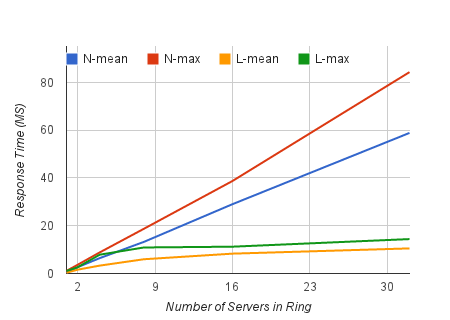
\includegraphics[width=1\columnwidth]{./response2.png}
\caption{$O(N)$ vs $O(\log N)$ Lookup}
\label{fig:finger-tables}
\end{figure}

\begin{figure}[h]
\vspace{-0.1in}
\centering
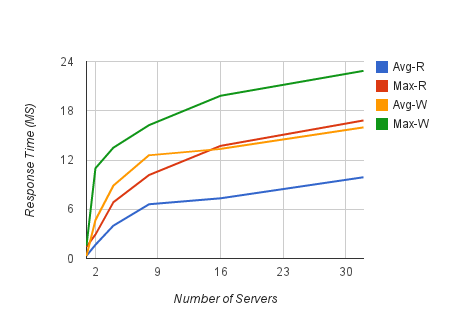
\includegraphics[width=1\columnwidth]{./response1.png}
\caption{Read vs. Write with Replication.}
\label{fig:read-write-rep}
\end{figure}

\paragraph{Over the network}
We run the same set of experiments, but now over the network. Each node is now hosted on a separate server (when the number of nodes exceeds the number of servers at our disposal, we run with a maximum of two nodes at each server). Figure \ref{} presents the results. As expected, the network does not have any other effect on the results presented above, other than adding latency to each of them.
For the rest of the experiments, we use implementations that incorporate finger tables.

\subsection{Concurrent lookups}
In this experiment, we analyze the effect of concurrent lookups on latency. We run the experiment with XX servers and YY clients, with each of them adding and retrieving ZZ keys from the nodes. The results are presented in Figure \ref{}.

\begin{figure}[h]
\centering
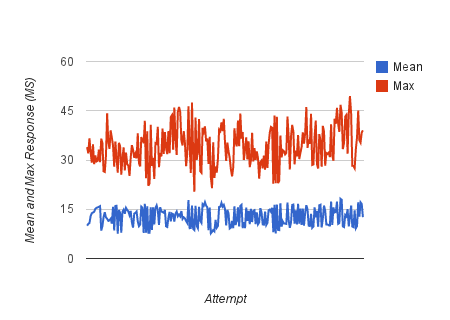
\includegraphics[width=1\columnwidth]{./contention.png}
\caption{Contention.}
\label{fig:contention}
\end{figure}



\subsection{Synchronous replication}

\subsection{Asynchronous replication}

\subsection{Node failures}

\begin{figure}[h]
\centering
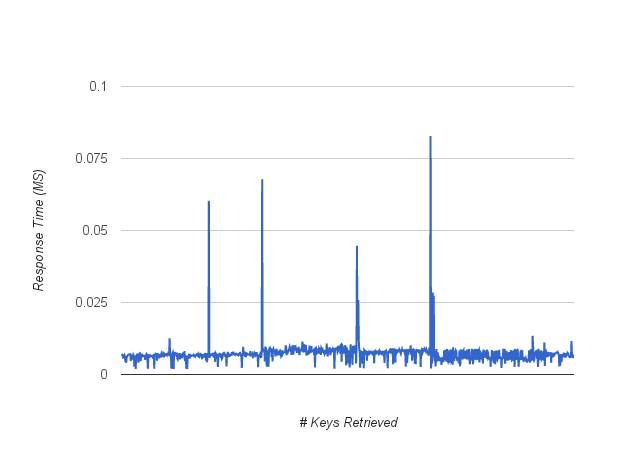
\includegraphics[width=1\columnwidth]{./response-fail.png}
\caption{Response Time on Server Failure}
\label{fig:response-fail}
\end{figure}


\section{Limitations}
Python threads...  bl

\section{Conclusion and future work}
We have implemented a scalable and fault tolerant distributed hash table based on Chord \cite{chord}. We experimented with different replication and lookup strategies and compared their performance. 

Beehive, Dynamo??

%\end{document}  % This is where a 'short' article might terminate


%
% The following two commands are all you need in the
% initial runs of your .tex file to
% produce the bibliography for the citations in your paper.
\vspace{-0.1cm}
\bibliographystyle{abbrv}
\begin{thebibliography}{00}
\vspace{-0.1cm}

\bibitem{chord}
I. Stoica, R. Morris, D. Karger, M. Frans Kaashoek, H. Balakrishnan
``A Scalable Peer-to-peer Lookup Service for Internet Applications",
{\em http://pdos.lcs.mit.edu/chord} (2001)

\bibitem{consistenthashing}
D. Karger, E. Lehman, F. Leighton, M. Levine, D. Lewin and R. Panigrahy,
``Consistent hashing and random trees: Distributed caching protocols for relieving hot spots on the World Wide Web."
{\em Proceedings of the 29th Annual ACM Symposium on Theory of Computing} (1997)

  % sigproc.bib is the name of the Bibliography in this case
% You must have a proper ".bib" file
%  and remember to run:
% latex bibtex latex latex
% to resolve all references
%
% ACM needs 'a single self-contained file'!
%
% That's all folks!
\end{thebibliography}
\end{document}